\chapter{性能评测}
\section{实验环境及方法}
我们在16台戴尔R720服务器上评估ClickNP的性能。每个FPGA都通过2个以太网端口与机架顶(top-of-rack, ToR)的戴尔S6000交换机相连。
我们在Windows Server 2012 R2上运行ClickNP。对于在Linux上运行的软件网络功能,我们使用CentOS 7.2平台,其内核版本为3.10。

为了测量网络功能的延迟,我们通过端口2将处理得到的包转发至回声(Echo)服务器。
回声服务器的FPGA中烧有回声逻辑,将收到的包发回其来源。
我们据此比较从端口1收到包起至从端口2收到回声包的时间差,得到精确到纳秒的延迟时长。
回声造成的延迟可以预先校正。

在我们的实验中,测试流量由包生成器PktGen产生,在包大小恒定为64字节时,
生成包的速率最高达到54.8Mpps。

\section{数据吞吐率及处理延迟评估}
\subsection{OpenFlow防火墙}
我们在实验中将OpenFlow防火墙与Linux防火墙以及Click+DPDK进行对比。
Linux防火墙采用IPSet处理精确匹配规则,采用IPTables处理模糊匹配规则。
我们在结果中引入了所使用的戴尔S6000交换机的性能作为参照,其防火墙处理能力有限,
只支持1.7K条模糊匹配规则。

值得一提的是,原先的Click+DPDK不支持接收端扩放(receive side scaling, RSS)。
我们在实验中修复了这一问题,而且发现Click+DPDK只需要4个核就可达到其最佳性能。
与此同时,对于Linux防火墙,我们需要尽可能地增加核数来提升其性能。
然而接收端扩放的限制使其最多只能使用8个核。

图~\ref{fig:ofwrate} 展示各防火墙在不同数量模糊匹配规则下的处理速率对比。
可见ClickNP和S6000均可达到56.4Mpps的最大速率。

Click+DPDK的处理速率大约可达18Mpps。Click采用了静态决策树来实现模糊匹配,因而其处理速率不随规则增多而降低。
然而该决策树的实现需要基于所有规则的先验知识,在运行时更新规则很困难。

基于IPTable的Linux防火墙处理速率低达2.67Mpps。
而且因为IPTable的模糊匹配是线性的,所以其处理速率随着规则的增多呈倒数级下降。
\begin{figure}[ht]
\centering
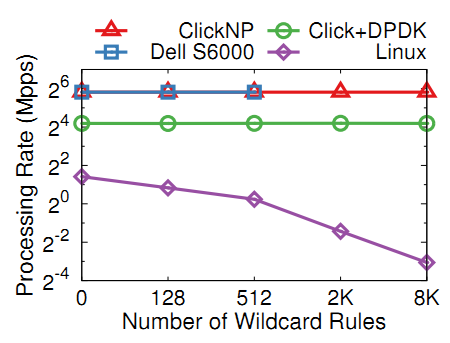
\includegraphics[width=4in]{ofwrate}
\caption{各防火墙模糊匹配速率对比} \label{fig:ofwrate}
\note{包大小为64字节}
\end{figure}

图~\ref{fig:ofwlatload} 展示各防火墙在不同负载下的小包处理延迟。
鉴于不同防火墙的处理能力差别明显,我们根据系统最大处理速率将负载标准化处理。
据图可见,在各个负载下,FPGA (ClickNP)和专用集成电路(S6000)的延迟均保持在2微秒以下,
相比之下软件处理的延迟大得多且不稳定,例如在高负载下Click+DPDK的延迟甚至高达50微秒。
\begin{figure}[ht]
\centering
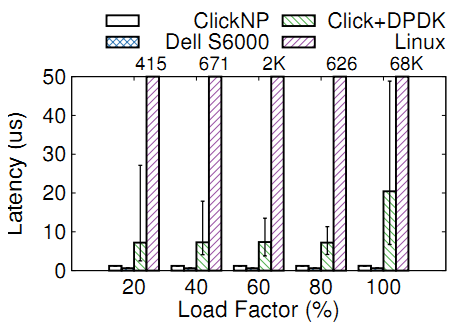
\includegraphics[width=4in]{ofwlatload}
\caption{不同负载下防火墙处理延迟对比} \label{fig:ofwlatload}
\note{包大小为64字节,误差杆置信水平为90\%}
\end{figure}
